\section{Simulazione}

TODO: rivdere questa introduzione (io la rivedrei)

Data la straordinarietà degli eventi che erano in corso dal punto di vista sanitario nel nostro paese si è reso necessario svolgere gran parte del lavoro in modalità a distanza e quindi senza la possibilità di testare il modello matematico appena ottenuto e i successivi risultati dovuti all'azione di controllo sul V.A.B., il lavoro quindi è stato svolto per la maggior parte sfruttando il tool \textit{Simulink} di Matlab che è, in poche parole, un risolutore di equazioni differenziali.

Abbiamo così adottato una metodologia di lavoro basata su prototipi sempre più simili a quello che dovrebbe essere il sistema reale.

Si va ora ad analizzare la risposta del sistema al controllo ottenuto nei punti precedenti, per assicurarci, che quanto scritto sopra valga oltre che nella teoria anche nella pratica:
\begin{figure}[H]
	\centering   	
	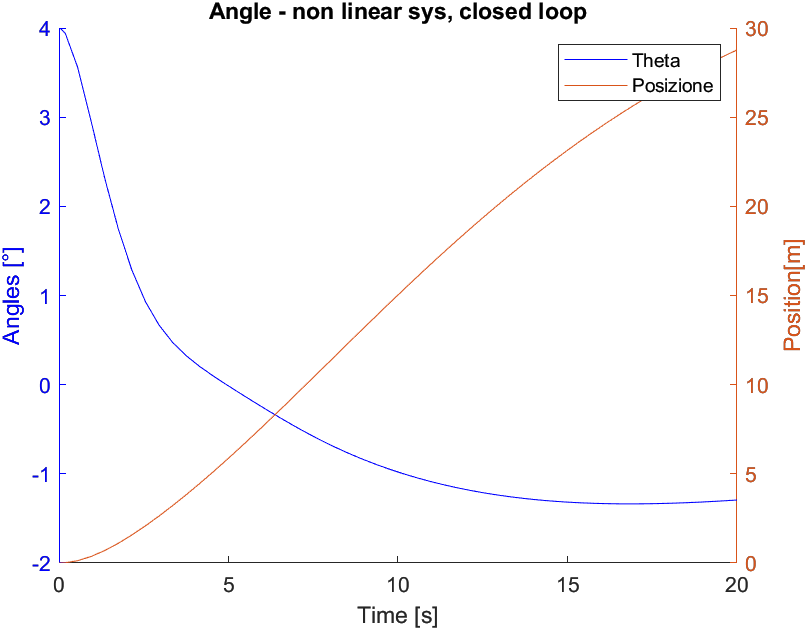
\includegraphics[width=0.7\textwidth]{Immagini/closed_loop_non_linear.png}
	\caption{Risposta del sistema non lineare in anello chiuso}
	\label{fig:closed_loop_non_linear_response}
\end{figure}
\begin{figure}[H]
	\centering   	
	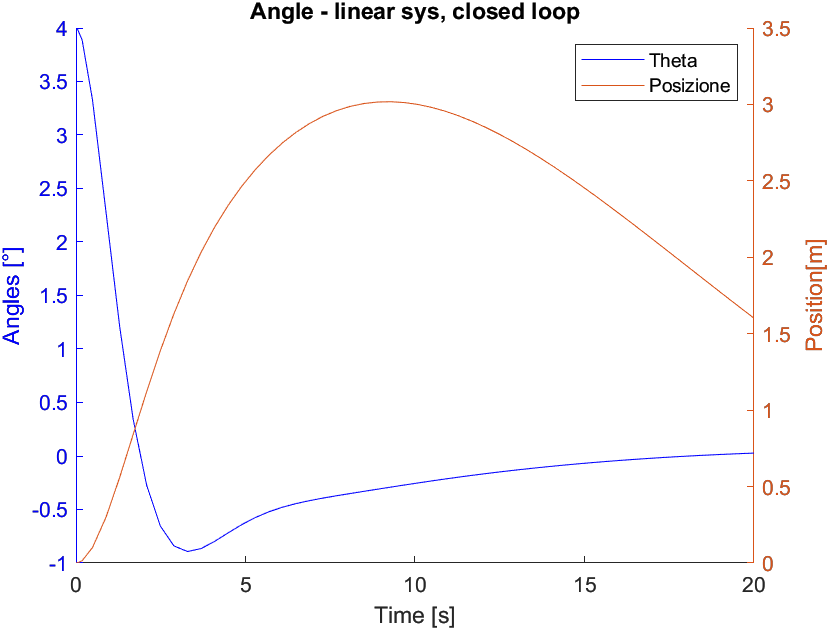
\includegraphics[width=0.7\textwidth]{Immagini/closed_loop_linear.png}
	\caption{Risposta del sistema lineare in anello chiuso}
	\label{fig:closed_loop_linear_response}
\end{figure}
TODO: come spieghiamo la differenza? rifare la simulazione?



\subsection{Simulazione del sistema non lineare}

Il primo compito che abbiamo risolto è stato quello di implementare le equazioni differenziali ottenute nel capitolo precedente:
\begin{itemize}
	\item $\ddot{\phi} = f_{\ddot{\phi}} (M_c,\theta,\dot{\theta},C_m)$
	\item $\ddot{\theta} = f_{\ddot{\theta}} (M_c,\theta,\dot{\theta},C_m)$
\end{itemize}

Dove $M_c$ sarebbe la massa del passeggero, $\theta e \dot{\theta}$ lo stato del sistema e $C_m$  la coppia erogata dal motore. Si può notare come entrambe le equazioni differenziali siano indipendenti dalla coordinata libera $\phi$.
\begin{figure}[H]
	\centering   	
	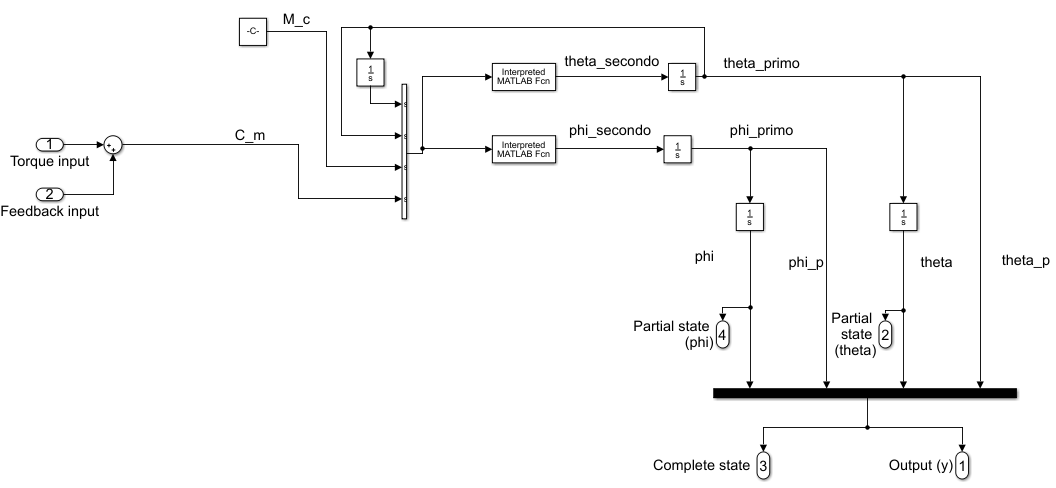
\includegraphics[width=1\textwidth]{Immagini/non_linear_system.png}
	\caption{Implementazione simulink delle equazioni differenziali}
	\label{fig:non_linear_system}
\end{figure}
In Fig.\ref{fig:non_linear_system} le \textit{interpreted function} altro non sono che  $f_{\ddot{\phi}}$ e $f_{\ddot{\theta}}$. A valle di esse sono presenti degli integratori che permettono di ottenere lo stato $x$ completo del sistema. Si può facilmente notare come $\dot{\theta} e \theta$ siano collegate direttamente all'input delle \textit{interpreted function}.
Si è dunque proceduto a  simulare il sistema per verificare la bontà di quanto ottenuto; in particolare, il sistema in anello aperto, dovrebbe oscillare all'infinito vista la mancanza di attriti nel modello.

\begin{figure}[H]
	\centering   	
	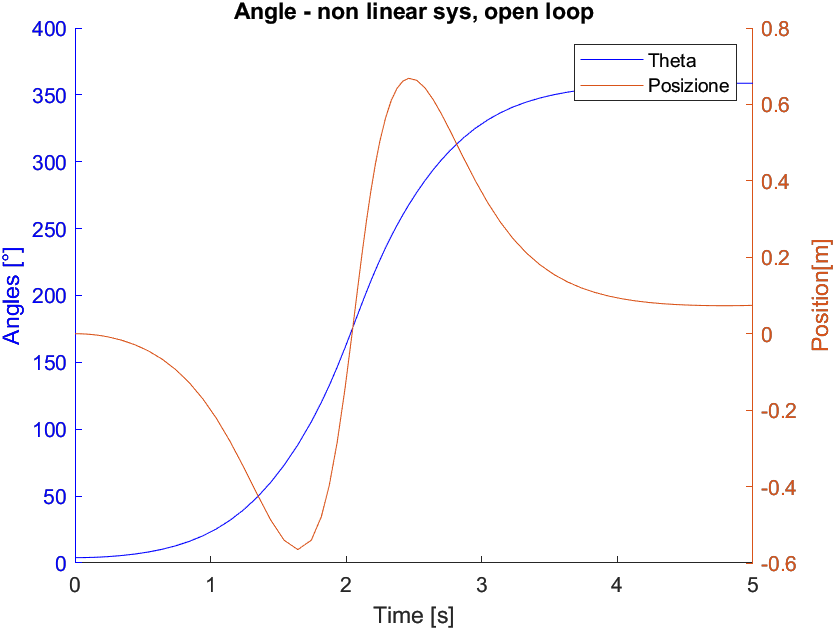
\includegraphics[width=0.6\textwidth]{Immagini/open_loop_response_non_linear.png}
	\caption{Risposta in anello aperto del sistema reale}
	\label{fig:open_loop_response_non_linear}
\end{figure}
La simulazione, il cui risultato è riportato in Fig.\ref{fig:open_loop_response_non_linear} è stata svolta per 5 secondi e con un angolo iniziale di 4°; il grafico mostra dunque l'andamento di $\theta$ nel tempo e della posizione che in termini matematici si esprime come $posizione = \phi \cdot{r_{ruota}}$
\label{sec:simulazione_reale}
\subsection{Simulazione del sistema lineare}
Si è inoltre creato un altro modello sfruttando il sistema lineare ottenuto prima  con l'obbiettivo di semplificare il problema e di velocizzare le simulazioni con lo scopo di testare rapidamente nuove tecniche di controllo che se avessero dato esito positivo sul modello lineare sarebbero poi state testate sul simulink che imita il comportamento reale del sistema.
\begin{figure}[H]
	\centering   	
	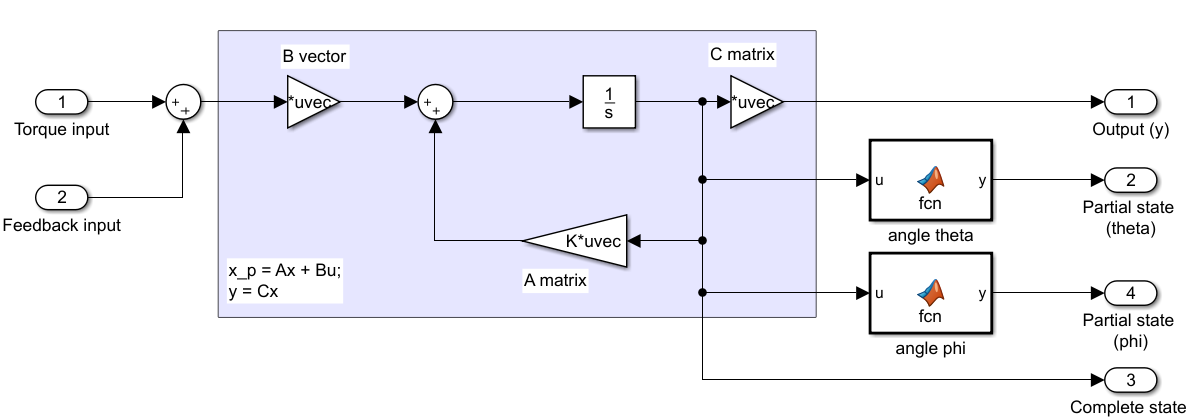
\includegraphics[width=1\textwidth]{Immagini/linear_system.png}
	\caption{Implementazione simulink del sistema linearizzato}
	\label{fig:linear_system}
\end{figure}

\begin{figure}[H]
	\centering   	
	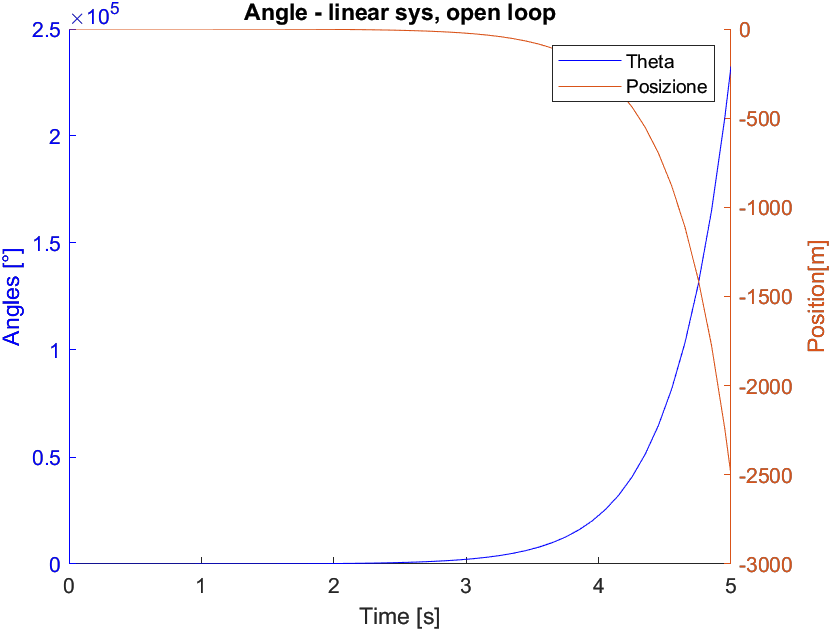
\includegraphics[width=0.6\textwidth]{Immagini/linear_open_loop.png}
	\caption{Risposta in anello aperto del sistema lineare}
	\label{fig:open_loop_response}
\end{figure}
In questo caso, la simulazione in anello aperto mostra che il sistema diverge; questo perché la linearizzazione ha senso attorno al punto di equilibrio da cui è stata ottenuta, distante da quel punto il sistema lineare non approssima più il sistema reale ed anche un eventuale controllo ottenuto da esso non garantisce buone performance distante da quel punto. Si nota, in Fig.\ref{fig:open_loop_response} che il punto di partenza è 4° e il sistema, lineare, diverga quasi immediatamente; la differenza con la risposta del sistema non lineare in Fig.\ref{fig:open_loop_response_non_linear}

Come già verificato in precedenza (sezione ~\ref{sec:open_loop_analysis}) ci sono due poli reali, uno negativo e uno positivo; questo dimostra come il sistema sia instabile in anello aperto e necessiti di controllo.

\subsection{Motore}
Il passo successivo è stato quello di andare a modellizzare il motore presente a bordo dello chassis; questo è necessario in quanto si deve tenere conto, in primo luogo, del ritardo che gli attuatori ( cioè il motore) introducono nel sistema e che per questo potrebbe diventare instabile.
\begin{figure}[H]
	\centering   	
	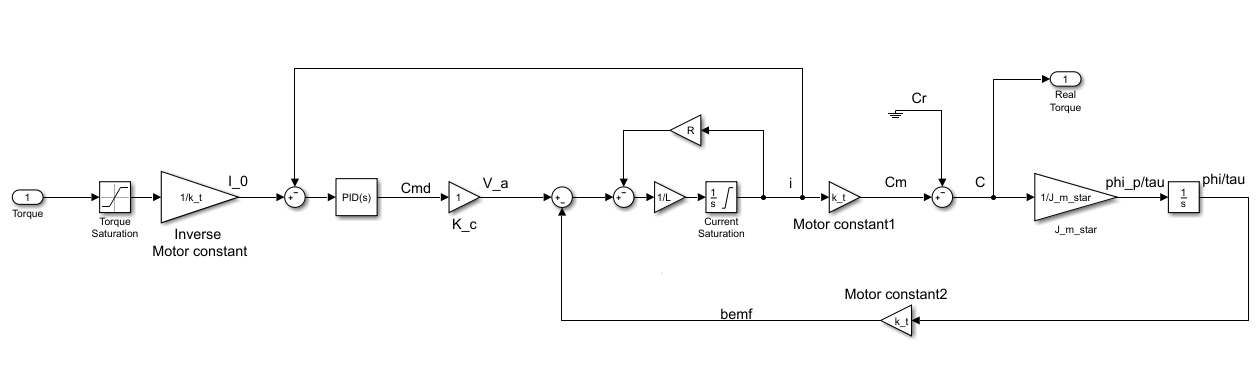
\includegraphics[width=1\textwidth]{Immagini/motor.png}
	\caption{Schema a blocchi del motore}
	\label{fig:motor}
\end{figure}

I valori delle componenti in Fig.\ref{fig:motor} sono presi dal datasheet del motore.
Il controllo del motore DC in questione e stato ottenuto tramite una retroazione in corrente che permette quindi di definire un setpoint alla corrente presente nel motore. Questo si è reso necessario poiché il controllore, attraverso il vettore K e lo stato del sistema, definisce la coppia che il motore dovrebbe erogare. In un motore DC la correlazione tra coppia erogata e corrente esiste ed è ben definita e si tratta di $k_t$.
Il controllore è stato realizzato seguendo metodi già noti in letteratura TODO: scrivere la formula o trovare un posto che la spieghi 
\begin{figure}[H]
	\centering   	
	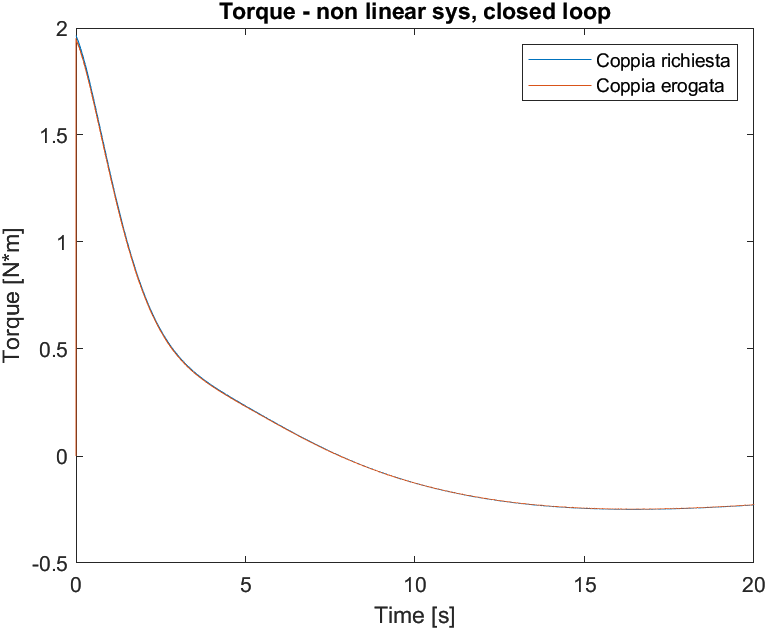
\includegraphics[width=0.7\textwidth]{Immagini/motore.png}
	\caption{Transitorio del motore}
	\label{fig:motore}
\end{figure}
\begin{figure}[H]
	\centering   	
	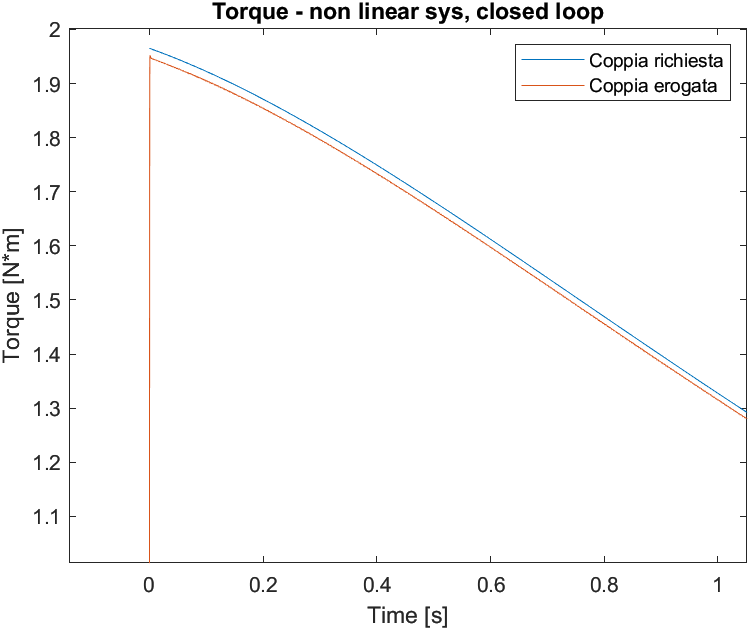
\includegraphics[width=0.7\textwidth]{Immagini/motore_zoom.png}
	\caption{Zoom del grafico in figura Fig.\ref{fig:motore}}
	\label{fig:motore_zoom}
\end{figure}

Come si può notare il picco di coppia massimo è minore di 2; questo è dovuto al fatto che, per ragioni esterne, nel motore può scorrere ua corrente di massimo 20A e quindi:
\begin{center}
	$C_{m,max} = I_{max}\cdot{K_{motore}} = 20 A\cdot{10 \dfrac{N\cdot{m}}{A}}=2N\cdot{m}$
\end{center}

Un esempio in cui la coppia richiesta supera i $2N\cdot{m}$ è il seguente:
\begin{figure}[H]
	\centering   	
	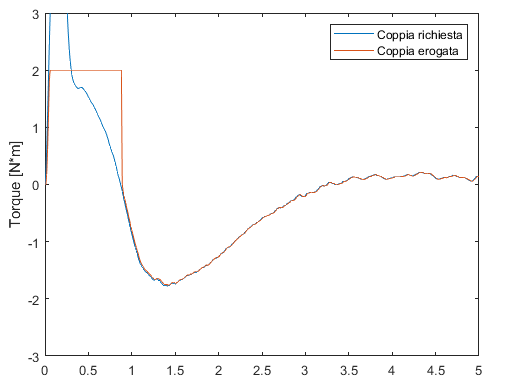
\includegraphics[width=0.8\textwidth]{Immagini/saturazione.png}
	\caption{Clamp della coppia erogata da parte del motore}
	\label{fig:clamp_motore}
\end{figure}
In Fig.\ref{fig:clamp_motore} è anche possibile notare come l'assenza del blocchetto denominato \textit{Torque saturation}, presente in Fig.\ref{fig:motor}, satura l'azione integrale dell'attuatore e inserisce un ritardo non secondario nell'azione di controllo.
\subsection{Modello complessivo (al momento)}
L'obbiettivo di questo paragrafo è quello di fare il punto della situazione del sistema sviluppato fino a questo punto e di sviluppare alcune considerazioni sul lavoro fatto.

\begin{figure}[H]
	\centering   	
	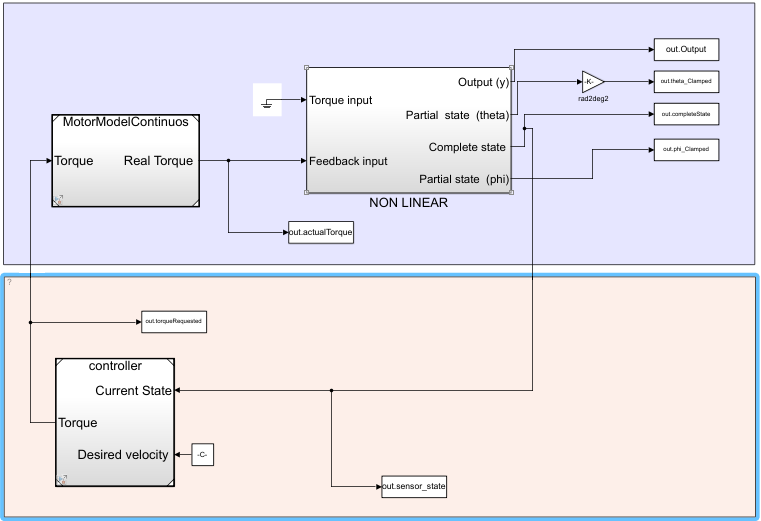
\includegraphics[width=0.8\textwidth]{Immagini/simulink_model_continuos.png}
	\caption{Simulink}
	\label{fig:simulink}
\end{figure}
Come si osserva in Fig.\ref{fig:simulink} il sistema al momento comprende tre blocchi:
\begin{itemize}
	\item Il blocco \textit{non linear}: rappresenta quello che nella realtà sarebbe il sistema reale; si occupa durante la simulazione, dati gli input, di restituire output simili a quelli che si avrebbero in laboratorio utilizzando la macchina vera e propria.
	\item Il blocco \textit{MotorModelContinuos}: si occupa di simulare la presenza e i transitori dovuti ai motori che nella realtà sono posti a bordo dello chassis.
	\item Il blocco \textit{controller}: è, dei tre, l'unico blocco che effettivamente dovrebbe essere implementato su un calcolatore. Con i valori simulati dai due blocchi di cui sopra calcola il valore di coppia per il controllo e lo fornisce indietro ai suddetti blocchi per completare la retroazione.
\end{itemize}
Il sistema al momento è, in linea teorica, a tempo continuo. Nella realtà in un computer e in particolar modo su Simulink la possibilità di far operare i blocchi che simulano il sistema reale a tempo continuo è preclusa.
Si é scelto dunque,per quanto fatto finora, di lasciare scegliere al software di Simulink il passo della simulazione ed in particolar modo utilizzare un passo variabile. Questo permette, nei punti in cui le variazioni sono spiccate(ad esempio quando il sistema si avvia) di utilizzare un passo di simulazione anche dell'ordine dei nanosecondi che approssima quasi perfettamente l'esecuzione a tempo continuo.

\subsection{Discretizzazione}
Come già detto sopra, il controllore è necessario che sia implementato su u calcolatore e quindi verrà eseguito a tempo discreto; per tenere conto di questa caratteristica è necessario discretizzare il controllore e acquisire gli input a tempo discreto:
\begin{itemize}
	\item all'ingresso del blocco \textit{controller} è stato posto un \textit{Sample \& Holder}; questo blocco si occupa di acquisire ogni tempo di sampling $T_s$ il valore in input e mantenerlo inalterato fino alla lettura successiva
	\item all'uscita del \textit{controller} si è posizionato un altro \textit{Sample \& Holder} per le stesse ragioni
	\item il \textit{controller} è stato trasformato a tempo discreto; TODO inseriamo la cosa dei poli discreti o diciamo che sono uguali essendo un proporzionale?
	A differenza del controllore della retroazione dello stato, il controllore che chiude la retroazione in velocità va ricalcolato tenendo conto del $T_s$; fortunatamente Simulink fa da solo questa conversione se si setta il blocco simulink \textit{Controllore PID} come integratore a tempo discreto fornendo il $T_s$ e la costante moltiplicativa.
\end{itemize}
Il controllore a tempo discreto ha dunque questo aspetto nel modello simulink implementato:
\begin{figure}[H]
	\centering   	
	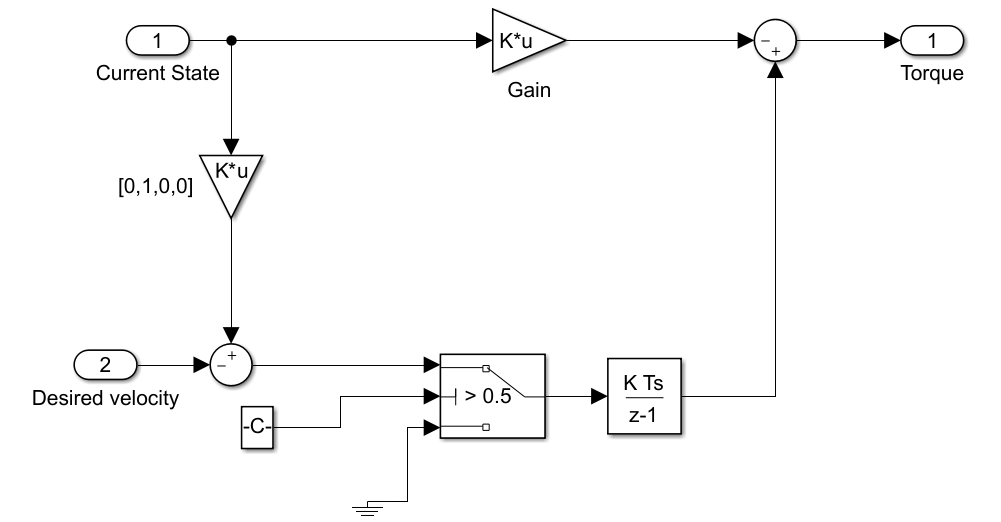
\includegraphics[width=0.8\textwidth]{Immagini/controller_discrete.png}
	\caption{Modello Simulink del controllore}
	\label{fig:controller_discrete}
\end{figure}